% Created 2018-06-21 Thu 12:30
\documentclass[8pt]{beamer}
\usepackage[sc,osf]{mathpazo}   % With old-style figures and real smallcaps.
\linespread{1.025}              % Palatino leads a little more leading
% Euler for math and numbers
\usepackage[euler-digits,small]{eulervm}
%\documentclass[10pt]{llncs}
%\usepackage{llncsdoc}
\usepackage{hyperref}
\usepackage{minted}
%\usemintedstyle{xcode}
\usepackage[utf8]{inputenc}
\usepackage[T1]{fontenc}
\usepackage{fixltx2e}
\usepackage{graphicx}
\usepackage{longtable}
\usepackage{float}
\usepackage{wrapfig}
\usepackage{rotating}
\usepackage[normalem]{ulem}
\usepackage{amsmath}
\usepackage{textcomp}
\usepackage{marvosym}
\usepackage{wasysym}
\usepackage{amssymb}
\usepackage{polynom}
\usepackage{changepage}
\usepackage{lipsum}


\hypersetup{colorlinks=true,
    linkcolor = blue,
    urlcolor  = blue,
    citecolor = blue,
    anchorcolor = blue
}
\renewcommand{\mod}[1]{\left( \texttt{mod}~#1 \right)}
\newcommand{\cpp}[1]{\mintinline{cpp}{#1}}
\newcommand{\py}[1]{\mintinline{py}{#1}}
\newcommand{\raw}[1]{\mintinline{text}{#1}}
\newcommand{\hs}[1]{\mintinline{hs}{#1}}
\newcommand{\smallpt}{\texttt{smallpt}}
\newcommand{\Ray}{\texttt{Ray}}
\newcommand{\Refl}{\texttt{Refl}}
\newcommand{\main}{\texttt{main}}
\newcommand{\intersect}{\texttt{intersect}}
\newcommand{\intersects}{\texttt{intersects}}
\tolerance=1000
\usetheme{Antibes}
\author{Davean Scies, Siddharth Bhat}
\date{November 4th, 2020}
\institute{Haskell Exchange}
\title{Optimizing \smallpt}
\hypersetup{
  pdfkeywords={},
  pdfsubject={},
  pdfcreator={Emacs 24.5.1 (Org mode 8.2.10)}}

  \usepackage{xcolor}

\usepackage{listings}

\newcommand{\lstbg}[3][0pt]{{\fboxsep#1\colorbox{#2}{\strut #3}}}
\lstdefinelanguage{diff}{
  basicstyle=\ttfamily\small,
  morecomment=[f][\lstbg{red!20}]-,
  morecomment=[f][\lstbg{green!20}]+,
  morecomment=[f][\textit]{@@},
  %morecomment=[f][\textit]{---},
  %morecomment=[f][\textit]{+++},
}


\begin{document}

\maketitle

\begin{frame}[fragile]{What is smallpt anyway?}
\pause
\begin{columns}
\begin{column}{0.48\textwidth}
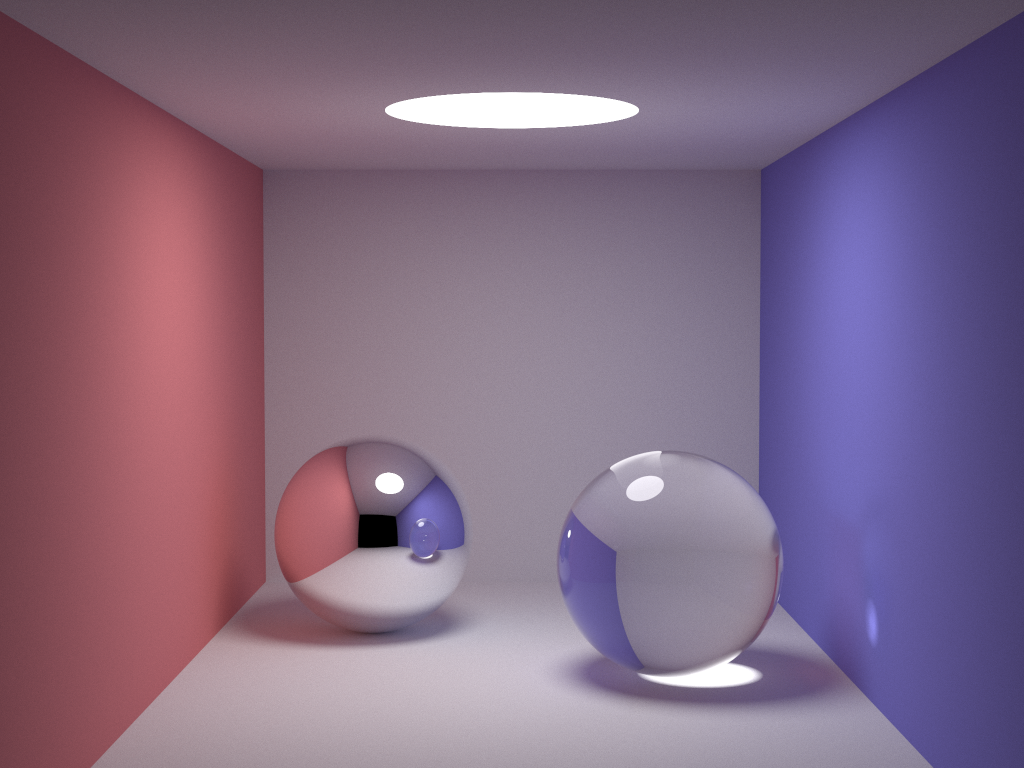
\includegraphics[height=0.8\textwidth]{./smallpt-render.png}
\end{column}
\begin{column}{0.48\textwidth}
\pause
\begin{itemize}
\item 100 LoC C demo of a raytracer \pause
\item Perfect for an optimization case study
\end{itemize}
\end{column}
\end{columns}
\end{frame}

\begin{frame}[fragile]{What is smallpt anyway?}
% \begin{adjustwidth}{-5em}{-5em}
\begin{minted}{cpp}
#include <math.h>
#include <stdlib.h>
#include <stdio.h>
struct Vec {      
  double x, y, z; // position, also color (r,g,b) 
  ... methods...
}; 
struct Ray { Vec o, d; Ray(Vec o_, Vec d_) : o(o_), d(d_) {} }; 
enum Refl_t { DIFF, SPEC, REFR };  // material types, used in radiance() 
struct Sphere { 
  double rad;   // radius 
  Vec p, e, c;  // position, emission, color 
  Refl_t refl;  // reflection type (DIFFuse, SPECular, REFRactive) 
  ... methods ...
  double intersect(const Ray &r) const // returns distance, 0 if nohit 
}; 
Sphere spheres[] = {//Scene: radius, position, emission, color, material 
  Sphere(1e5, Vec( 1e5+1,40.8,81.6), Vec(),Vec(.75,.25,.25),DIFF),//Left 
  ... initialization ...
}; 
inline bool intersect(const Ray &r, double &t, int &id) 
\end{minted}
% \end{adjustwidth}
\end{frame}


\begin{frame}[fragile]{What is smallpt anyway?}
\footnotesize
\begin{minted}{cpp}
Vec radiance(const Ray &r, int depth, unsigned short *Xi){ 
  double t;                               // distance to intersection 
  int id=0;                               // id of intersected object 
  if (!intersect(r, t, id)) return Vec(); // if miss, return black 
  const Sphere &obj = spheres[id];        // the hit object 
  Vec x=r.o+r.d*t, n=(x-obj.p).norm(), nl=n.dot(r.d)<0?n:n*-1, f=obj.c; 
  double p = f.x>f.y && f.x>f.z ? f.x : f.y>f.z ? f.y : f.z; // max refl 
  if (++depth>5) if (erand48(Xi)<p) f=f*(1/p); else return obj.e; //R.R. 
  if (obj.refl == DIFF){                  // Ideal DIFFUSE reflection 
    double r1=2*M_PI*erand48(Xi), r2=erand48(Xi), r2s=sqrt(r2); 
    Vec w=nl, u=((fabs(w.x)>.1?Vec(0,1):Vec(1))%w).norm(), v=w%u; 
    Vec d = (u*cos(r1)*r2s + v*sin(r1)*r2s + w*sqrt(1-r2)).norm(); 
    return obj.e + f.mult(radiance(Ray(x,d),depth,Xi)); 
  } else if (obj.refl == SPEC)            // Ideal SPECULAR reflection 
    return obj.e + f.mult(radiance(Ray(x,r.d-n*2*n.dot(r.d)),depth,Xi)); 
  Ray reflRay(x, r.d-n*2*n.dot(r.d));     // Ideal dielectric REFRACTION 
  bool into = n.dot(nl)>0;                // Ray from outside going in? 
  double nc=1, nt=1.5, nnt=into?nc/nt:nt/nc, ddn=r.d.dot(nl), cos2t; 
  if ((cos2t=1-nnt*nnt*(1-ddn*ddn))<0)    // Total internal reflection 
    return obj.e + f.mult(radiance(reflRay,depth,Xi)); 
  Vec tdir = (r.d*nnt - n*((into?1:-1)*(ddn*nnt+sqrt(cos2t)))).norm(); 
  double a=nt-nc, b=nt+nc, R0=a*a/(b*b), c = 1-(into?-ddn:tdir.dot(n)); 
  double Re=R0+(1-R0)*c*c*c*c*c,Tr=1-Re,P=.25+.5*Re,RP=Re/P,TP=Tr/(1-P); 
  return obj.e + f.mult(depth>2 ? (erand48(Xi)<P ?   // Russian roulette 
    radiance(reflRay,depth,Xi)*RP:radiance(Ray(x,tdir),depth,Xi)*TP) : 
    radiance(reflRay,depth,Xi)*Re+radiance(Ray(x,tdir),depth,Xi)*Tr); 
} 
\end{minted}
\end{frame}

\begin{frame}[fragile]{Establishing baselines}
\begin{minted}{hs}
main :: IO ()
main = smallptM 200 200 256

smallptM :: Int -> Int -> Int -> IO ()
smallptM !w !h !nsamps = do
  -- ... processing
  withFile "image.ppm" WriteMode $ \hdl -> do
        hPrintf hdl "P3\n%d %d\n%d\n" w h (255::Int)
        flip mapM_ [0..w*h-1] $ \i -> do
          Vec r g b <- VM.unsafeRead c i
          hPrintf hdl "%d %d %d " (toInt r) (toInt g) (toInt b)
\end{minted}

\pause
\begin{itemize}
\item \raw{Sha256} hash of the output image (deterministic)
\end{itemize}

\end{frame}

\begin{frame}[fragile]{Haskell: the first stab}
How do we communicate the code? x(

{\tiny
\begin{minted}{hs}
radiance :: Ray -> CInt -> Ptr CUShort -> IO Vec
radiance ray@(Ray o d) depth xi =
 case intersects ray of
  (Nothing,_) -> return zerov
  (Just (D# t),Sphere r p e c refl) -> do
    let x = addv o (mulvs d t)
        n = norm $ x `subv` p
        nl = if isTrue# ((dot n d) <## 0.0##) then n else mulvs n (-1.0##)
        pr = maxv c
        depth' = depth + 1
        continue f = case refl of
          DIFF -> do
            (CDouble (D# r)) <- erand48 xi
            let r1 = (2.0## *## 3.141592653589793238##) *##  r
            (CDouble (D# r2)) <- erand48 xi
            let r2s = sqrtDouble# r2
                w@(Vec wx _ _) = nl
                u = norm (cross (if isTrue# (fabsDouble# wx >## 0.1##) then (Vec 0.0## 1.0## 0.0##) else (Vec 1.0## 0.0## 0.0##)) w)
                v = w `cross` u
                d' = norm $ (u`mulvs`(cosDouble# r1*##r2s)) `addv` (v`mulvs`(sinDouble# r1*##r2s)) `addv` (w`mulvs`sqrtDouble# (1.0## -##r2))
            rad <- radiance (Ray x d') depth' xi
            return $ e `addv` (f `mulv` rad)

          SPEC -> do
            let d' = d `subv` (n `mulvs` (2.0## *## (n`dot`d)))
            rad <- radiance (Ray x d') depth' xi
            return $ e `addv` (f `mulv` rad)

          REFR -> do
            let reflRay = Ray x (d `subv` (n `mulvs` (2.0## *## n`dot`d))) -- Ideal dielectric REFRACTION
                into = n`dot`nl >## 0.0##                -- Ray from outside going in?
                nc = 1.0##
                nt = 1.5##
                nnt = if isTrue# into then nc/##nt else nt/##nc
                ddn= d`dot`nl
                cos2t = 1.0##-##nnt*##nnt*##(1.0## -##ddn*##ddn)
            if isTrue# (cos2t<##0.0##)    -- Total internal reflection
              then do
                rad <- radiance reflRay depth' xi
                return $ e `addv` (f `mulv` rad)
              else do
                let tdir = norm (d`mulvs`nnt `subv` (n`mulvs`((if isTrue# into then 1.0## else -1.0##)*##(ddn*##nnt+##sqrtDouble# cos2t))))
                    a=nt-##nc
                    b=nt+##nc
                    r0=a*##a/##(b*##b)
                    c = 1.0## -## (if isTrue# into then -1.0## *## ddn else tdir`dot`n)
                    re=r0 +## (1.0## -## r0) *## c *## c*## c *## c *## c 
                    tr=1.0## -## re
                    pp=0.25## +## 0.5## *## re
                    rp=re /## pp
                    tp=tr /## (1.0## -## pp)
                rad <-
                  if (depth > 2 )
                    then do (CDouble (D# er)) <- erand48 xi
                            if isTrue# (er<##pp) -- Russian roulette
                              then (`mulvs` rp) `fmap` radiance reflRay depth' xi
                              else (`mulvs` tp) `fmap` radiance (Ray x tdir) depth' xi
                    else do rad0 <- (`mulvs` re) `fmap` radiance reflRay depth' xi
                            rad1 <- (`mulvs` tr) `fmap` radiance(Ray x tdir) depth' xi
                            return $ rad0 `addv` rad1
                return $ e `addv` (f `mulv` rad)

    if depth'>5
      then do
        (CDouble (D# er)) <- erand48 xi
        if isTrue# (er <## pr) then continue $ c `mulvs` (1.0## /## pr)
                  else return e
      else continue 
\end{minted}
}
\end{frame}


\begin{frame}[fragile]{Optimisation 1: manual unrolling + unboxing }
\end{frame}

\begin{frame}[fragile]{Optimisation 2: Optimizing \Ray}
\end{frame}

\begin{frame}[fragile]{Optimisation 3: Newtyping \Refl}
\end{frame}

\begin{frame}[fragile]{Optimisation 4: Unbox tuple of \intersects}
\end{frame}


\begin{frame}[fragile]{Optimisation 3: Only expose \main}
\end{frame}


\begin{frame}[fragile]{Optimisation 3: Strictify \intersect}
\end{frame}


\begin{frame}[fragile]{Optimisation ...: Enable LLVM}
\begin{columns}
\begin{column}{0.48\textwidth}
{\footnotesize
\begin{minted}{diff}
diff --git a/smallpt-hs.cabal b/smallpt-hs.cabal
index 83ec118..64d2788 100644
--- a/smallpt-hs.cabal
+++ b/smallpt-hs.cabal
@@ -26,4 +26,5 @@ executable smallpt-hs
                        vector

   -- no -Wall as type signature are purposely missing
+  ghc-options:         -O2 -rtsopts -fllvm
-  ghc-options:         -O2 
\end{minted}
}
\end{column}
\begin{column}{0.48\textwidth}
Perf delta here
\end{column}
\end{columns}
\end{frame}


\begin{frame}[fragile]{Takeaways}
\pause
\begin{itemize}
\item Haskell can be fast \pause
\item ... with a lot of work! \pause
\item Accumulate optimizations to accrue performance wins. \pause
\item \href{https://docs.google.com/spreadsheets/d/1YhZlDRGvnCtN8UQf_0ItmgRWI9MhL21HDTlBEKqgWHc/edit#gid=0}{Raw Google Sheet of our transformations}
\item \href{https://github.com/bollu/smallpths}{\texttt{github.com/bollu/smallpt-opt}}
\end{itemize}
\end{frame}
\end{document}
